\documentclass[11pt]{article}
% Shared preamble for the printable mini lessons (1.4 onward).
%   \documentclass[11pt]{article}
%   \input{../preamble}
% Build the key with:  pdflatex -jobname=<name>_KEY "\def\iskey{}\input{<name>}"
% Figures shared with the web page live in figures/Unit_X/<name>.tex and are
% pulled in with \fig{Unit_X/<name>}; the standalone package drops their own
% preamble, so their macros come from figures/preamble.tex, loaded here.
% Shared preamble for web figures.  Each figure is a standalone .tex that
% \input's this file; scripts/make-figures.sh turns it into an SVG.
\usepackage[T1]{fontenc}
\usepackage{helvet}
\renewcommand{\familydefault}{\sfdefault}
\usepackage{tikz}
\usetikzlibrary{decorations.pathreplacing}
% axis numbers in the text font, not math italic
\pgfkeys{/pgf/number format/.cd,assume math mode=true,1000 sep={}}

% dot plot: \dotplot{min}{max}{value/count,...}{axis label}
\newcommand{\dotplot}[4]{%
\begin{tikzpicture}[x=0.9cm,y=0.33cm]
  \draw[thick] (#1-0.5,0) -- (#2+0.5,0);
  \foreach \t in {#1,...,#2} {\draw (\t,0.25) -- (\t,-0.25) node[below] {\t};}
  \foreach \v/\c in {#3} {\ifnum\c>0 \foreach \k in {1,...,\c} {\fill (\v,\k*1.15) circle (0.16cm);}\fi}
  \node at ({(#1+#2)/2},-2.3) {#4};
\end{tikzpicture}}

% shape sketch histogram (12 bins): \shapehist{heights}{label}
\newcommand{\shapehist}[2]{%
  \foreach \h [count=\i from 0] in {#1} \draw[fill=gray!30] (\i,0) rectangle (\i+1,\h);
  \draw (-0.3,0) -- (12.3,0);
  \node[font=\bfseries] at (6,-2.6) {#2};}
\newcommand{\meanmark}[1]{\fill (#1,0) -- ++(-0.3,-0.75) -- ++(0.6,0) -- cycle;}
\newcommand{\medmark}[2]{\draw[very thick,dashed] (#1,0) -- (#1,#2);}

% number line with minor ticks: \nline{min}{max}{label step}{axis label}
\newcommand{\nline}[4]{%
  \draw[thick] (#1-0.5,0) -- (#2+0.5,0);
  \foreach \t in {#1,...,#2} \draw (\t,0.12) -- (\t,-0.12);
  \pgfmathtruncatemacro{\nxt}{#1+#3}
  \foreach \t in {#1,\nxt,...,#2} \draw (\t,0.2) -- (\t,-0.2) node[below] {\t};
  \node at ({(#1+#2)/2},-0.95) {#4};}
% box plot above the line: \bplot{min}{Q1}{med}{Q3}{max}
\newcommand{\bplot}[5]{%
  \draw[thick] (#1,1.0) -- (#2,1.0);
  \draw[thick] (#4,1.0) -- (#5,1.0);
  \draw[thick] (#1,0.75) -- (#1,1.25);
  \draw[thick] (#5,0.75) -- (#5,1.25);
  \draw[thick,fill=gray!20] (#2,0.55) rectangle (#4,1.45);
  \draw[very thick] (#3,0.55) -- (#3,1.45);}

% ---- added for 1.4 onward ----
% axis on y=0: \axis{min}{max}{label step}{tick step}{axis label}
\newcommand{\axis}[5]{%
  \draw[thick] (#1,0) -- (#2,0);
  \pgfmathsetmacro{\axT}{#1+#4}\foreach \t in {#1,\axT,...,#2} \draw (\t,0.1) -- (\t,-0.1);
  \pgfmathsetmacro{\axL}{#1+#3}\foreach \t in {#1,\axL,...,#2}
    \draw (\t,0.18) -- (\t,-0.18) node[below] {\pgfmathprintnumber{\t}};
  \node at ({(#1+#2)/2},-0.95) {#5};}
% box plot centred at height y: \bplotat{y}{min}{Q1}{med}{Q3}{max}
\newcommand{\bplotat}[6]{%
  \draw[thick] (#2,#1) -- (#3,#1);
  \draw[thick] (#5,#1) -- (#6,#1);
  \draw[thick] (#2,#1-0.22) -- (#2,#1+0.22);
  \draw[thick] (#6,#1-0.22) -- (#6,#1+0.22);
  \draw[thick,fill=gray!20] (#3,#1-0.42) rectangle (#5,#1+0.42);
  \draw[very thick] (#4,#1-0.42) -- (#4,#1+0.42);}
% an outlier dot: \outlier{x}{y}
\newcommand{\outlier}[2]{\fill (#1,#2) circle (2.4pt);}

\usepackage[margin=0.75in]{geometry}
\usepackage{array}
\usepackage{enumitem}
\usepackage{amsmath}
\usepackage[helvet]{sfmath}  % math in the same sans font as the text
\usepackage{standalone}
\pagestyle{empty}
\setlength{\parindent}{0pt}
\setlist[enumerate,1]{leftmargin=1.5em,itemsep=1em}
\setlist[enumerate,2]{label=(\alph*),leftmargin=2em,itemsep=2.2em}

\newif\ifkey
\ifdefined\iskey \keytrue \fi
\colorlet{keyred}{red!75!black}
\newcommand{\ans}[1]{\ifkey\leavevmode{\color{keyred}#1}\fi}
% vertical work space on the student copy, less on the key
\newcommand{\work}[1]{\ifkey\vspace{0.6em}\else\vspace{#1}\fi}
\newcommand{\fig}[1]{\input{../../figures/#1}}
% Title line: \lessontitle{Quartiles, IQR, and Box Plots}
\newcommand{\lessontitle}[1]{{\Large\bfseries #1\ifkey\ \textcolor{keyred}{KEY}\fi}\hfill Name \underline{\hspace{2in}}\par\vspace{0.6em}}
\newcommand{\partner}{\par\vspace{0.4em}Work with a partner. Compare answers when you finish each problem.\par}

% Unit quiz: two questions per mini lesson, each headed by the lesson's
% objective.  The key keeps every box the same height as the student copy,
% so key page N lines up with quiz page N.
% 2.5 and 2.6 use the printed z-table (handouts/Unit_2/Z_Table.tex); key
% answers use its 4-decimal areas, and a reverse lookup takes the closest area.
\newcommand{\lessonhead}[1]{\par\vspace{0.6em}{\large\bfseries #1}\par\vspace{0.25em}\hrule\vspace{0.6em}}
\newcommand{\goal}[1]{\textbf{#1}\par\vspace{0.35em}}
% answer box: same height on both copies, answer printed only on the key
\newcommand{\abox}[2]{\par\begin{minipage}[t][#1][t]{\linewidth}\raggedright\vspace{0.2em}\ans{#2}\end{minipage}\par}
% circle a choice on the left, explain in a fixed-height box on the right:
% \pick{choices}{box height}{key answer}
\newcommand{\pick}[3]{\par\vspace{0.3em}\begin{minipage}[t]{2.45in}\vspace{0pt}#1\end{minipage}\hfill
  \begin{minipage}[t][#2][t]{3.9in}\vspace{0pt}\raggedright Explain: \ans{#3}\end{minipage}\par}
% circled choices: \opt{A} prints plain; \optans{B} is circled in red on the key
\newcommand{\opt}[1]{\tikz[baseline=(c.base)]\node[rounded corners=0.6em,inner sep=2.5pt](c){#1};}
\newcommand{\optans}[1]{\ifkey\tikz[baseline=(c.base)]\node[rounded corners=0.6em,inner sep=2.5pt,draw=keyred,thick,text=keyred](c){#1};\else\opt{#1}\fi}
% one row of an SD table (as in 2.1): \sdrow{x}{x - mean}{(x - mean)^2}; the last two show on the key only
\newcommand{\sdrow}[3]{#1 & \ans{#2} & \ans{#3} \\ \hline}
\newenvironment{sdtable}{\renewcommand{\arraystretch}{1.45}\begin{tabular}{|c|p{1.0in}|p{1.0in}|}\hline
  $x$ & $x - \bar{x}$ & $(x - \bar{x})^2$ \\ \hline}{\end{tabular}}
\setlist[enumerate,2]{label=(\alph*),leftmargin=2em,itemsep=0.3em}
\setlist[enumerate,1]{leftmargin=1.5em,itemsep=1em}
\raggedright\hyphenpenalty=10000\exhyphenpenalty=10000

\begin{document}

\lessontitle{Unit 2 Quiz: Analyzing One Variable}

Show your work.

% ======================================================================
\lessonhead{2.1 - Standard Deviation}
\begin{enumerate}

\item \goal{I find the standard deviation of a small data set.}
Kim counted how many text messages she got each hour for 5 hours.
\begin{center}2,\; 6,\; 0,\; 4,\; 3\end{center}
\begin{minipage}[t]{0.5\linewidth}\vspace{0pt}\raggedright
\begin{enumerate}
  \item Find the mean, $\bar{x}$. Then complete the table.

  \vspace{0.5em}
  $\bar{x} =$ \underline{\makebox[1.3in]{\ans{$15 \div 5 = 3$}}}

  \vspace{0.6em}
  \begin{sdtable}
  \sdrow{2}{$-1$}{1}
  \sdrow{6}{3}{9}
  \sdrow{0}{$-3$}{9}
  \sdrow{4}{1}{1}
  \sdrow{3}{0}{0}
  \multicolumn{2}{|r|}{$\Sigma(x - \bar{x})^2$} & \ans{20} \\ \hline
  \end{sdtable}
\end{enumerate}
\end{minipage}\hfill
\begin{minipage}[t]{0.47\linewidth}\vspace{0pt}\raggedright
\begin{enumerate}[start=2]
  \item Find the standard deviation, $s$. Round to 2 decimal places.
  \abox{8em}{$s = \sqrt{\frac{\Sigma(x - \bar{x})^2}{n - 1}} = \sqrt{\frac{20}{4}}$\\[0.5em]
  $= \sqrt{5} \approx 2.24$ messages}
\end{enumerate}
\end{minipage}

\item \goal{I compare the spread of data sets by looking at graphs, and I explain what the standard deviation tells about data.}
These dot plots show the goals two soccer teams scored in 8 games. Both teams have a mean of 3 goals.

\vspace{0.3em}
\begin{minipage}[t]{0.45\linewidth}\vspace{0pt}\raggedright
\begin{tikzpicture}[x=0.95cm,y=1cm]
  \begin{scope}[yshift=2.9cm]
    \axis{0}{6}{1}{1}{}
    \dotsat{2/1,3/6,4/1}
    \node[anchor=east,font=\small\bfseries] at (-0.3,0.6) {Team A};
  \end{scope}
  \axis{0}{6}{1}{1}{Goals in a game}
  \dotsat{0/1,1/1,2/1,3/2,4/1,5/1,6/1}
  \node[anchor=east,font=\small\bfseries] at (-0.3,0.6) {Team B};
\end{tikzpicture}
\end{minipage}\hfill
\begin{minipage}[t]{0.52\linewidth}\vspace{0pt}\raggedright
\begin{enumerate}
  \item Which team has the larger standard deviation? Explain.
  \abox{3.4em}{Team B. Its goals are spread far from 3. Team A's goals are packed close to 3.}
  \item Team B's SD is 2 goals. What does this number tell you about Team B?
  \abox{3.4em}{Team B's goals in a game are usually about 2 goals away from its mean of 3.}
  \item Team C scored exactly 3 goals in every game. What is Team C's SD? Explain.
  \abox{3.4em}{0. Every value is the same as the mean, so there is no spread.}
\end{enumerate}
\end{minipage}

\end{enumerate}

% ======================================================================
\newpage
\lessonhead{2.2 - Choosing Measures and Comparing Distributions}
\begin{enumerate}[resume]

\item \goal{I choose mean and SD or median and IQR based on the shape of the data.}
For each data set, circle the measures you should use. Then explain.
\begin{enumerate}[itemsep=0.5em]
  \item The minutes 30 students spent on the bus today. The histogram is skewed right.
  \pick{\opt{mean and SD}\hspace{1em}\optans{median and IQR}}{2.4em}{The data is skewed.}
  \item The lengths of 100 leaves from one tree. The histogram is symmetric, with no outliers.
  \pick{\optans{mean and SD}\hspace{1em}\opt{median and IQR}}{2.4em}{The data is symmetric with no outliers.}
  \item The prices of 7 used phones, in dollars: \; 120,\; 140,\; 150,\; 150,\; 160,\; 180,\; 450
  \pick{\opt{mean and SD}\hspace{1em}\optans{median and IQR}}{3.8em}{450 is an outlier. (Q1 $= 140$, Q3 $= 180$, IQR $= 40$, upper fence $= 180 + 60 = 240$.) It pulls the mean and the SD.}
\end{enumerate}

\item \goal{I compare two distributions using shape, center, spread, and outliers.}
These dot plots show how many hours students in two clubs practiced last week.

\vspace{0.3em}
\begin{minipage}[t]{0.58\linewidth}\vspace{0pt}\raggedright
\begin{tikzpicture}[x=0.64cm,y=1cm]
  \begin{scope}[yshift=2.8cm]
    \axis{0}{12}{1}{1}{}
    \dotsat{2/1,3/1,4/2,5/3,6/2,7/3,8/2,9/1,10/1}
    \node[anchor=east,font=\small\bfseries] at (-0.3,0.6) {Soccer};
  \end{scope}
  \axis{0}{12}{1}{1}{Hours practiced last week}
  \dotsat{1/2,2/5,3/4,4/2,5/2,11/1}
  \node[anchor=east,font=\small\bfseries] at (-0.3,0.6) {Chess};
\end{tikzpicture}
\end{minipage}\hfill
\begin{minipage}[t]{0.38\linewidth}\vspace{0pt}\raggedright
\renewcommand{\arraystretch}{1.35}
\begin{tabular}{|l|c|c|c|c|}\hline
 & Q1 & Median & Q3 & IQR \\ \hline
Soccer & 4.5 & 6 & 7.5 & 3 \\ \hline
Chess & 2 & 3 & 4 & 2 \\ \hline
\end{tabular}
\begin{enumerate}
  \item Describe the shape of each club's data.
  \abox{3em}{Soccer is symmetric.\\ Chess is skewed right.}
\end{enumerate}
\end{minipage}

\vspace{0.4em}
\begin{enumerate}[start=2]
  \item Compare the centers. Use numbers and the context.
  \abox{3em}{The median for soccer (6 hours) is greater than for chess (3 hours). Soccer players usually practiced 3 hours more.}
  \item Compare the spreads. Use numbers.
  \abox{3em}{The IQR for soccer (3 hours) is greater than for chess (2 hours). The middle half of the soccer players is more spread out.}
  \item Does either club have an outlier? Explain.
  \abox{3em}{Yes. One chess player practiced 11 hours. The upper fence for chess is $4 + 1.5 \times 2 = 7$, and 11 is above 7.}
\end{enumerate}

\end{enumerate}

% ======================================================================
\newpage
\lessonhead{2.3 - Percentiles and Z-Scores}
\begin{enumerate}[resume]

\item \goal{I find the percentile of a value.}
20 students said how many minutes they played a phone game last night. Here are the times, in order.
\begin{center}5,\; 8,\; 12,\; 15,\; 18,\; 20,\; 22,\; 25,\; 27,\; 30,\; 32,\; 35,\; 38,\; 40,\; 42,\; 45,\; 50,\; 55,\; 60,\; 75\end{center}
\begin{enumerate}
  \item What percentile is 45 minutes?
  \abox{3.6em}{15 times are below 45. \quad $15 \div 20 = 0.75$, the 75th percentile}
  \item What percentile is 15 minutes?
  \abox{3.6em}{3 times are below 15. \quad $3 \div 20 = 0.15$, the 15th percentile}
  \item Which time is at the 40th percentile?
  \abox{3.6em}{40\% of 20 is 8 times below it. The 9th time is \textbf{27 minutes}.}
\end{enumerate}

\item \goal{I find and explain a z-score, and I compare values from different data sets with z-scores.}
Amina took two tests.

\begin{center}
\renewcommand{\arraystretch}{1.3}
\begin{tabular}{|l|c|c|c|}\hline
Test & Amina's score & Class mean $\mu$ & Class SD $\sigma$ \\ \hline
Math & 79 & 73 & 4 \\ \hline
Reading & 91 & 83 & 8 \\ \hline
\end{tabular}
\end{center}
\begin{enumerate}
  \item Find Amina's z-score on each test.
  \abox{5em}{Math: \; $z = \frac{x - \mu}{\sigma} = \frac{79 - 73}{4} = \frac{6}{4} = 1.5$ \qquad Reading: \; $z = \frac{91 - 83}{8} = \frac{8}{8} = 1$}
  \item What does Amina's z-score on the math test tell you?
  \abox{3em}{Her math score is 1.5 standard deviations above the class mean.}
  \item Amina's reading score is higher. On which test did she do better compared to her class? Explain.
  \abox{3.6em}{Math. Her z-score on math (1.5) is larger than her z-score on reading (1).}
\end{enumerate}

\end{enumerate}

% ======================================================================
\newpage
\lessonhead{2.4 - Normal Distributions and the Empirical Rule}
\begin{enumerate}[resume]

\item \goal{I use the empirical rule (68-95-99.7) to find percents, and I find the percentile of a value 1, 2, or 3 SDs from the mean.}
The high temperature each day in July in one city has a normal distribution. The mean is 88$^\circ$F and the SD is 4$^\circ$F.

\vspace{0.3em}
\begin{minipage}[t]{0.5\linewidth}\vspace{0pt}\raggedright
\begin{enumerate}
  \item Label the number line with the temperatures.

  \vspace{0.5em}
  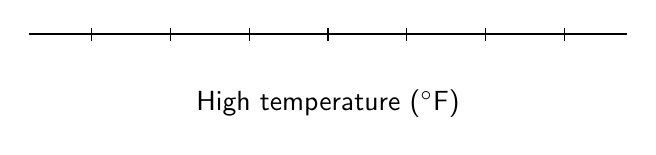
\begin{tikzpicture}[x=1.0cm,y=0.65cm]
    \bellcurve
    \draw[thick] (-3.8,0) -- (3.8,0);
    \foreach \z in {-3,...,3} \draw (\z,0.12) -- (\z,-0.12);
    \ifkey\begin{scope}[keyred]\foreach \z/\v in {-3/76,-2/80,-1/84,0/88,1/92,2/96,3/100} \node[below] at (\z,-0.12) {\v};\end{scope}\fi
    \node at (0,-1.35) {High temperature ($^\circ$F)};
  \end{tikzpicture}
  \item About what percent of days have a high temperature from 84$^\circ$F to 92$^\circ$F?
  \abox{2em}{68\% (within 1 SD)}
\end{enumerate}
\end{minipage}\hfill
\begin{minipage}[t]{0.47\linewidth}\vspace{0pt}\raggedright
\begin{enumerate}[start=3]
  \item About what percent of days have a high temperature above 96$^\circ$F?
  \abox{2em}{$2.35 + 0.15 = 2.5\%$}
  \item About what percent of days have a high temperature from 80$^\circ$F to 92$^\circ$F?
  \abox{2em}{$13.5 + 34 + 34 = 81.5\%$}
  \item What percentile is a high temperature of 92$^\circ$F?
  \abox{3em}{92 is 1 SD above the mean.\\ $50 + 34 = 84$, the 84th percentile}
\end{enumerate}
\end{minipage}

\item \goal{I describe a normal distribution, and I compare normal curves with different means and SDs.}
The three curves are normal distributions.

\vspace{0.3em}
\begin{minipage}[t]{0.52\linewidth}\vspace{0pt}\raggedright
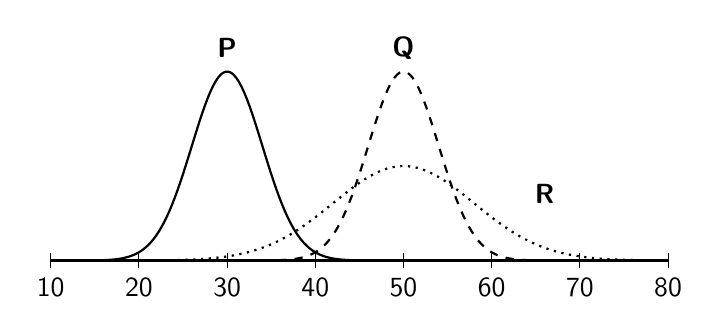
\begin{tikzpicture}[x=0.112cm,y=1cm]
  \draw[thick] (10,0) -- (80,0);
  \foreach \t in {10,20,...,80} {\draw (\t,0.1) -- (\t,-0.1) node[below] {\t};}
  \draw[thick,domain=12:48,samples=120] plot (\x,{2.4*exp(-(\x-30)*(\x-30)/32)});
  \draw[thick,dashed,domain=32:68,samples=120] plot (\x,{2.4*exp(-(\x-50)*(\x-50)/32)});
  \draw[thick,dotted,domain=20:80,samples=150] plot (\x,{1.2*exp(-(\x-50)*(\x-50)/128)});
  \node[font=\bfseries] at (30,2.7) {P};
  \node[font=\bfseries] at (50,2.7) {Q};
  \node[font=\bfseries] at (66,0.85) {R};
\end{tikzpicture}
\end{minipage}\hfill
\begin{minipage}[t]{0.45\linewidth}\vspace{0pt}\raggedright
\begin{enumerate}
  \item Which two curves have the same mean?
  \abox{1.8em}{Q and R (both 50)}
  \item Which two curves have the same SD?
  \abox{1.8em}{P and Q (same width and shape)}
  \item Which curve has the largest SD? Explain.
  \abox{2.8em}{R. It is the widest and most spread out.}
\end{enumerate}
\end{minipage}

\begin{enumerate}[start=4]
  \item Which statement is true for every normal distribution? Circle the letter.

  \vspace{0.3em}
  \begin{tabular}{@{}l@{\hspace{0.4em}}p{2.75in}l@{\hspace{0.4em}}l}
  \opt{A} & The mean is greater than the median. & \optans{B} & The mean and the median are equal.\\[0.3em]
  \opt{C} & The data is skewed right. & \opt{D} & The mean is always 0.\\
  \end{tabular}
\end{enumerate}

\end{enumerate}

% ======================================================================
\newpage
\lessonhead{2.5 - Normal Calculations with a Z-Table}
Use the z-table.
\begin{enumerate}[resume]

\item \goal{I read a z-table.}
\begin{minipage}[t]{0.48\linewidth}\vspace{0pt}\raggedright
Find the area \textbf{below} each z-score.
\begin{enumerate}
  \item $z = 0.73$
  \abox{3em}{.7673}
  \item $z = -1.45$
  \abox{3em}{.0735}
\end{enumerate}
\end{minipage}\hfill
\begin{minipage}[t]{0.48\linewidth}\vspace{0pt}\raggedright
Find the area \textbf{above} or \textbf{between}.
\begin{enumerate}[start=3]
  \item above $z = 1.10$
  \abox{3em}{$1 - .8643 = .1357$}
  \item between $z = -1.30$ and $z = 0.40$
  \abox{3em}{$.6554 - .0968 = .5586$}
\end{enumerate}
\end{minipage}

\item \goal{I find the percent of data below, above, or between values in a normal distribution.}
A machine fills bottles with water. The amounts have a normal distribution with a mean of 500 mL and an SD of 6 mL. What percent of the bottles have:
\begin{enumerate}
  \item less than 510 mL?
  \abox{7.5em}{$z = \frac{510 - 500}{6} = 1.67$. \quad Table: .9525. \quad \textbf{95.25\%}}
  \item more than 491 mL?
  \abox{7.5em}{$z = \frac{491 - 500}{6} = -1.5$. \quad Table: .0668. \quad $1 - .0668 = .9332$. \quad \textbf{93.32\%}}
  \item from 497 mL to 509 mL?
  \abox{8em}{$z = \frac{497 - 500}{6} = -0.5$, table .3085. \quad $z = \frac{509 - 500}{6} = 1.5$, table .9332.\\[0.4em]
  $.9332 - .3085 = .6247$. \quad \textbf{62.47\%}}
\end{enumerate}

\end{enumerate}

% ======================================================================
\newpage
\lessonhead{2.6 - Normal Calculations in Reverse}
Use the z-table.
\begin{enumerate}[resume]

\item \goal{I find the z-score for a percentile with the z-table, and I find the value at a percentile in a normal distribution.}
\begin{minipage}[t]{0.48\linewidth}\vspace{0pt}\raggedright
\begin{enumerate}
  \item Find the z-score at the 60th percentile.
  \abox{4em}{Closest area .5987: \; $z = 0.25$}
\end{enumerate}
\end{minipage}\hfill
\begin{minipage}[t]{0.48\linewidth}\vspace{0pt}\raggedright
\begin{enumerate}[start=2]
  \item Find the z-score at the 45th percentile.
  \abox{4em}{Closest area .4483: \; $z = -0.13$}
\end{enumerate}
\end{minipage}

\vspace{0.4em}
Scores in a video game have a normal distribution. The mean is 1,200 points and the SD is 200 points.
\begin{enumerate}[start=3]
  \item What score is at the 35th percentile?
  \abox{8em}{Area .3500. Closest area .3483: \; $z = -0.39$\\[0.4em]
  $x = \mu + z\sigma = 1200 + (-0.39)(200) = 1200 - 78 = 1122$ points}
\end{enumerate}

\item \goal{I find cutoffs for ``top'' and ``bottom'' percents.}
The weights of a bakery's loaves of bread have a normal distribution. The mean is 680 grams and the SD is 12 grams.
\begin{enumerate}
  \item The lightest 4\% of the loaves are sold at a lower price. Below what weight is a loaf sold at a lower price?
  \abox{9em}{Bottom 4\%: the area to the left is .0400. Closest area .0401: \; $z = -1.75$\\[0.4em]
  $680 + (-1.75)(12) = 680 - 21 = 659$ grams}
  \item The heaviest 30\% of the loaves get a ``large'' sticker. How heavy must a loaf be to get the sticker?
  \abox{9em}{Top 30\%: the area to the left is $1 - .30 = .70$. Closest area .6985: \; $z = 0.52$\\[0.4em]
  $680 + 0.52 \times 12 = 680 + 6.24 = 686.24$. \; About \textbf{686.2 grams}}
\end{enumerate}

\end{enumerate}

\end{document}
